\tikzstyle{inner} = [thin, circle, minimum size = 0.6cm, draw, inner sep = 0.1pt, black, font = \scriptsize]
\tikzstyle{inner_g} = [thin, circle, minimum size = 0.6cm, draw, inner sep = 0.1pt, black, fill = green]
\tikzstyle{inner_r} = [thin, circle, minimum size = 0.6cm, draw, inner sep = 0.1pt, black, fill = red]
\tikzstyle{inner_b} = [
	thin, circle, minimum size = 0.6cm, draw, inner sep = 0.1pt, black, fill = blue!30!white, font =
    \scriptsize]
\tikzstyle{ed} = [thick, ->, draw, black]

    
\begin{tikzpicture}

    \only<-1>{
        \node[inner] (a) at (0, 0) {$D_{17}$};
	}
    \only<2->{
        \node[inner_b] (a) at (0, 0) {$D_{17}$};
    }

    \only<-2>{
        \node[inner] (b) at (-1.5, -1) {$D_{16}$};
	}
    \only<3->{
        \node[inner_b] (b) at (-1.5, -1) {$D_{16}$};
    }
  

    \node[inner] (c) at (1.5, -1) {$D_{15}$};

    \node[inner] (d) at (-3, -2) {$D_{14}$};

    \only<-3>{
        \node[inner] (e) at (0, -2) {$D_{13}$};
	}
    \only<4->{
        \node[inner_b] (e) at (0, -2) {$D_{13}$};
    }

    \node[inner] (f) at (3, -2) {$D_{12}$};

    \node[inner] (g) at (-4.5, -3) {$D_{11}$};

    \only<-4>{
        \node[inner] (h) at (-1.5, -3) {$D_{10}$};
	}
    \only<5->{
        \node[inner_b] (h) at (-1.5, -3) {$D_{10}$};
    }

    \node[inner] (i) at (1.0, -3) {$D_9$};

    \only<-6>{
        \node[inner] (j) at (2.0, -3) {$D_8$};
	}
    \only<7->{
        \node[inner_b] (j) at (2.0, -3) {$D_8$};
    }

    \node[inner] (k) at (4.0, -3) {$D_7$};

    \only<-5>{
        \node[inner] (l) at (-2.5, -4) {$D_6$};
	}
    \only<6->{
        \node[inner_b] (l) at (-2.5, -4) {$D_6$};
    }

    \node[inner] (m) at (-0.5, -4) {$D_5$};

    \only<-7>{
        \node[inner] (n) at (1.2, -4) {$D_4$};
	}
    \only<8->{
        \node[inner_b] (n) at (1.2, -4) {$D_4$};
    }

    \node[inner] (o) at (2.8, -4) {$D_3$};

    \node[inner] (p) at (0.4, -5) {$D_2$};
    
    \only<-8>{
        \node[inner] (q) at (2, -5) {$D_1$};
	}
    \only<9->{
        \node[inner_b] (q) at (2, -5) {$D_1$};
    }


    
    \path (a) edge[ed] (b);
    \path (a) edge[ed] (c);
    \path (b) edge[ed] (d);
    \path (b) edge[ed] (e);
    \path (c) edge[ed] (e);
    \path (c) edge[ed] (f);
    \path (d) edge[ed] (g);
    \path (d) edge[ed] (h);
    \path (e) edge[ed] (h);
    \path (e) edge[ed] (i);
    \path (f) edge[ed] (j);
    \path (f) edge[ed] (k);
    \path (h) edge[ed] (l);
    \path (h) edge[ed] (m);
    \path (j) edge[ed] (n);
    \path (j) edge[ed] (o);
    \path (n) edge[ed] (p);
    \path (n) edge[ed] (q);
\end{tikzpicture}
